% Options for packages loaded elsewhere
\PassOptionsToPackage{unicode}{hyperref}
\PassOptionsToPackage{hyphens}{url}
\PassOptionsToPackage{dvipsnames,svgnames,x11names}{xcolor}
%
\documentclass[
  authoryear,
  preprint,
  3p]{elsarticle}

\usepackage{amsmath,amssymb}
\usepackage{lmodern}
\usepackage{iftex}
\ifPDFTeX
  \usepackage[T1]{fontenc}
  \usepackage[utf8]{inputenc}
  \usepackage{textcomp} % provide euro and other symbols
\else % if luatex or xetex
  \usepackage{unicode-math}
  \defaultfontfeatures{Scale=MatchLowercase}
  \defaultfontfeatures[\rmfamily]{Ligatures=TeX,Scale=1}
\fi
% Use upquote if available, for straight quotes in verbatim environments
\IfFileExists{upquote.sty}{\usepackage{upquote}}{}
\IfFileExists{microtype.sty}{% use microtype if available
  \usepackage[]{microtype}
  \UseMicrotypeSet[protrusion]{basicmath} % disable protrusion for tt fonts
}{}
\makeatletter
\@ifundefined{KOMAClassName}{% if non-KOMA class
  \IfFileExists{parskip.sty}{%
    \usepackage{parskip}
  }{% else
    \setlength{\parindent}{0pt}
    \setlength{\parskip}{6pt plus 2pt minus 1pt}}
}{% if KOMA class
  \KOMAoptions{parskip=half}}
\makeatother
\usepackage{xcolor}
\setlength{\emergencystretch}{3em} % prevent overfull lines
\setcounter{secnumdepth}{5}
% Make \paragraph and \subparagraph free-standing
\ifx\paragraph\undefined\else
  \let\oldparagraph\paragraph
  \renewcommand{\paragraph}[1]{\oldparagraph{#1}\mbox{}}
\fi
\ifx\subparagraph\undefined\else
  \let\oldsubparagraph\subparagraph
  \renewcommand{\subparagraph}[1]{\oldsubparagraph{#1}\mbox{}}
\fi


\providecommand{\tightlist}{%
  \setlength{\itemsep}{0pt}\setlength{\parskip}{0pt}}\usepackage{longtable,booktabs,array}
\usepackage{calc} % for calculating minipage widths
% Correct order of tables after \paragraph or \subparagraph
\usepackage{etoolbox}
\makeatletter
\patchcmd\longtable{\par}{\if@noskipsec\mbox{}\fi\par}{}{}
\makeatother
% Allow footnotes in longtable head/foot
\IfFileExists{footnotehyper.sty}{\usepackage{footnotehyper}}{\usepackage{footnote}}
\makesavenoteenv{longtable}
\usepackage{graphicx}
\makeatletter
\def\maxwidth{\ifdim\Gin@nat@width>\linewidth\linewidth\else\Gin@nat@width\fi}
\def\maxheight{\ifdim\Gin@nat@height>\textheight\textheight\else\Gin@nat@height\fi}
\makeatother
% Scale images if necessary, so that they will not overflow the page
% margins by default, and it is still possible to overwrite the defaults
% using explicit options in \includegraphics[width, height, ...]{}
\setkeys{Gin}{width=\maxwidth,height=\maxheight,keepaspectratio}
% Set default figure placement to htbp
\makeatletter
\def\fps@figure{htbp}
\makeatother

\usepackage{todonotes,mathtools}
\mathtoolsset{showonlyrefs}

\usepackage{booktabs}
\usepackage{longtable}
\usepackage{array}
\usepackage{multirow}
\usepackage{wrapfig}
\usepackage{float}
\usepackage{colortbl}
\usepackage{pdflscape}
\usepackage{tabu}
\usepackage{threeparttable}
\usepackage{threeparttablex}
\usepackage[normalem]{ulem}
\usepackage{makecell}
\usepackage{xcolor}
\makeatletter
\makeatother
\makeatletter
\makeatother
\makeatletter
\@ifpackageloaded{caption}{}{\usepackage{caption}}
\AtBeginDocument{%
\ifdefined\contentsname
  \renewcommand*\contentsname{Table of contents}
\else
  \newcommand\contentsname{Table of contents}
\fi
\ifdefined\listfigurename
  \renewcommand*\listfigurename{List of Figures}
\else
  \newcommand\listfigurename{List of Figures}
\fi
\ifdefined\listtablename
  \renewcommand*\listtablename{List of Tables}
\else
  \newcommand\listtablename{List of Tables}
\fi
\ifdefined\figurename
  \renewcommand*\figurename{Figure}
\else
  \newcommand\figurename{Figure}
\fi
\ifdefined\tablename
  \renewcommand*\tablename{Table}
\else
  \newcommand\tablename{Table}
\fi
}
\@ifpackageloaded{float}{}{\usepackage{float}}
\floatstyle{ruled}
\@ifundefined{c@chapter}{\newfloat{codelisting}{h}{lop}}{\newfloat{codelisting}{h}{lop}[chapter]}
\floatname{codelisting}{Listing}
\newcommand*\listoflistings{\listof{codelisting}{List of Listings}}
\makeatother
\makeatletter
\@ifpackageloaded{caption}{}{\usepackage{caption}}
\@ifpackageloaded{subcaption}{}{\usepackage{subcaption}}
\makeatother
\makeatletter
\@ifpackageloaded{tcolorbox}{}{\usepackage[many]{tcolorbox}}
\makeatother
\makeatletter
\@ifundefined{shadecolor}{\definecolor{shadecolor}{rgb}{.97, .97, .97}}
\makeatother
\makeatletter
\makeatother
\journal{Annals of Emergency Medicine}
\ifLuaTeX
  \usepackage{selnolig}  % disable illegal ligatures
\fi
\usepackage[]{natbib}
\bibliographystyle{elsarticle-harv}
\IfFileExists{bookmark.sty}{\usepackage{bookmark}}{\usepackage{hyperref}}
\IfFileExists{xurl.sty}{\usepackage{xurl}}{} % add URL line breaks if available
\urlstyle{same} % disable monospaced font for URLs
\hypersetup{
  pdftitle={Hierarchical time series forecasting in Emergency Medical Services},
  pdfauthor={Bahman Rostami-Tabar; Rob J. Hyndman},
  pdfkeywords={forecasting, healthcare, emergency services, forecast
reconciliation, hierarchical time series, ambulance demand, attended
incidents},
  colorlinks=true,
  linkcolor={blue},
  filecolor={Maroon},
  citecolor={Blue},
  urlcolor={Blue},
  pdfcreator={LaTeX via pandoc}}

\setlength{\parindent}{6pt}
\begin{document}

\begin{frontmatter}
\title{Hierarchical time series forecasting in Emergency Medical
Services}
\author[1]{Bahman Rostami-Tabar%
\corref{cor1}%
}
 \ead{rostami-tabarb@cardiff.ac.uk} 
\author[2]{Rob J. Hyndman%
%
}
 \ead{Rob.Hyndman@monash.edu} 

\affiliation[1]{organization={Cardiff University, Cardiff Business
School},country={United Kingdom},countrysep={,},postcode={CF10
3EU},postcodesep={}}
\affiliation[2]{organization={Monash University, Department of
Econometrics and Business
Statistics},country={Australia},countrysep={,},postcode={VIC
3800},postcodesep={}}

\cortext[cor1]{Corresponding author}


        
\begin{abstract}
Accurate forecasts of ambulance demand are crucial inputs when planning
and deploying staff and fleet. Such demand forecasts are required at
national, regional and sub-regional levels, and must take account of the
nature of incidents and their priorities. These forecasts are often
generated independently by different teams within the organization. As a
result, forecasts at different levels may be inconsistent, resulting in
conflicting decisions and a lack of coherent coordination in the
service. To address this issue, we exploit the hierarchical and grouped
structure of the demand time series, and apply forecast reconciliation
methods to generate both point and probabilistic forecasts that are
coherent and use all the available data at all levels of disaggregation.
The methods are applied to daily incident data from the Welsh Ambulance
Service NHS Trust, from October 2015 to July 2019, disaggregated by
nature of incident, priority, managing health board, and control area.
We use an ensemble of forecasting models, and show that the resulting
forecasts are better than any individual forecasting model. We validate
the forecasting approach using time-series cross-validation.
\end{abstract}





\begin{keyword}
    forecasting \sep healthcare \sep emergency services \sep forecast
reconciliation \sep hierarchical time series \sep ambulance demand \sep 
    attended incidents
\end{keyword}
\end{frontmatter}
    \ifdefined\Shaded\renewenvironment{Shaded}{\begin{tcolorbox}[boxrule=0pt, frame hidden, sharp corners, enhanced, interior hidden, borderline west={3pt}{0pt}{shadecolor}, breakable]}{\end{tcolorbox}}\fi

\hypertarget{sec-intro}{%
\section{Introduction}\label{sec-intro}}

Inability to match the resources with the demand in Emergency Medical
Services (EMS) results in an overcrowding care system. This is a serious
problem causing challenging situations on patient flow with serious
consequences on patients, staff and the entire care system
\citep{ekstrom2015forecasting, ROSTAMITABAR20221197}. Demand forecasting
in EMS is a vital element that helps to depict various courses of action
to avoid the mismatch, which can result in massive savings in terms of
patient safety and lives. An accurate daily demand forecasting enables
planners and decision makers to manage resources to meet anticipated
patients, reconfigure units, redeploy staff and vehicles, where
necessary.

Demand forecasts at EMS are typically required at multiple levels of
cross-sectional granularities to inform various planning and
decision-making processes \citep{hulshof2012taxonomic}. There are some
planning process at the national level (more strategic or long-term)
such as workforce resource planning and budgeting; sub-national,
regional or healthcare level (tactical or medium-term) such as temporary
capacity expansions, resource sharing and staff-shift scheduling; and
hospital or station level (operational or short-term) such as planning
rosters for staff and ambulance deployment. Demand forecasts might also
be required at different level for a specific group of interest such as
nature of demand or priority. Moreover, the time series data in EMS has
an inherent hierarchical and grouped structure to support such
forecasting requirements. Demand for emergency medical services at the
country level can be disaggregated in a geographical hierarchy into
sub-national, regions, health boards, stations/hospitals or divided into
groups such as nature of incidents or demand priority. Therefore, using
forecasting methodologies that account for hierarchical and/or grouped
structures of time series in EMS seems to be a natural fit.

However, despite a large number of studies dedicated to forecasting for
EMS
\citep{mingliterature2022, gul2020exhaustive, ibrahim2016modeling, wargon2009systematic},
this area is neglected and the main focus has been on producing
forecasts at a single level, independently. Generating independent
forecasts not only ignore the inherent hierarchical and/or grouped
structure relationships of the time series demand but also results in a
lack of consistency and coordination. Consistent forecasts of the EMS
demand across all hierarchical and grouped levels are paramount for an
effective planning and decision making. The hierarchical forecasting
approaches can not only create consistent forecasts but also achieve
more accurate forecasts than the independent (base) forecasts
\citep{hyndman2011optimal}. Obtaining consistent forecasts at different
levels is important as it helps to avoid making conflicting decisions.
With hierarchical forecasting, plans at any level are based on coherent
forecasts and therefore can be aligned. Implementing and sustaining
improvements in EMS require alignments and coordination between
different stakeholders, without which teams operate in isolation leading
to conflicts, duplication work, rework, or work that runs counter to the
overall goal to improve the quality of delivery service. Hierarchical
forecasting framework can be used as a tool to improve coordination
between teams across the care services at the national, sub-national,
regional and local levels. To our knowledge, there is not only no
research in the EMS forecasting to account for the hierarchical and
grouped structure of the system but also in the entire field of
forecasting for healthcare management.

In this paper, we address this gap by investigating the application of
hierarchical forecasting approaches in the EMS using daily time series
of verified incidents from 2015 to 2020 in a major ambulance service in
Great Britain. The data has hierarchical and grouped structures with
hierarchies at the national, control (i.e.~sub-national), health board
(i.e.~regional) and groups by priority and nature of incidents. We
produce not only the point forecast but also the forecast distribution
across all levels, which is critical for an effective planning and
associated risk management. We compare the point and probabilistic
forecast accuracy of the independent forecasts, bottom-up and optimal
reconciliation approaches. We first generate independent/based forecasts
using Exponential Smoothing State Space (ETS), Generalized Linear Model
(GLM), Poisson regression, a simple empirical distribution and an
ensemble method followed by applying bottom-up and optimal
reconciliation approaches. Forecast performance is assessed by the Root
Mean Squared Scaled Error (RMSSE) for point forecasts and the Continuous
Ranked Probability Score (CRPS) for the probabilistic forecasts. This
paper complies with the principles of the reproducibility
\citep{stodden2013best, boylan2015reproducibility}. Therefore, the study
could equally be applied to any healthcare service (e.g.~emergency
department, primary or social care) subject to the time series having a
hierarchical and/or grouped structure, which is generally the case in
the healthcare sector.

The remainder of this article is structured as follows: In section 2, we
provide a brief review of the literature and discuss its limitation to
position our work; in section 3, we present the experiment design
describing the data set, forecasting methods and forecast evaluation
metrics. In Section 4, we discuss the hierarchical time series
forecasting approaches to generate both point and probabilistic
forecasts. In section 5, we present and discuss our results; in section
7, we summarize our findings and present ideas for future research.

\hypertarget{lit}{%
\section{Research background}\label{lit}}

Emergency medical services (EMS) are a critical component in the
delivery of urgent medical care to communities. An effective service
delivery requires accurate resource planning that are generally replying
on demand forecasts at operational, tactical and strategic levels.

There is a substantial number of studies on the application of time
series forecasting in the Emergency Medical Services. Various areas have
been the focus of the literature. Forecasting call volume arrivals is
one of the major research topics. \citet{ibrahim2016modeling} provide an
extensive review of the forecasting models in this context. Another
important area is related to forecasting ambulance demand. Although the
definition of demand might not be always clearly stated, however, this
is typically referring to a situation where a physical resource has been
deployed to respond to an incident. This might be also called
\emph{attended incidents}. Another demand related variable is verified
incidents. These are all incidents that require an action: either send a
physical vehicle, deal with via the Clinical Support Desk (e.g.~calls),
get an external (private) provider to respond to it, or send it through
to other channels such as police, firefighters or general practitioners.
Our study is aligned with this stream of the literature. Another similar
area that is largely studied in the literature, is Emergency Department
forecasting. We refer interested readers to \citet{mingliterature2022},
\citet{gul2020exhaustive} and \citet{wargon2009systematic} for extensive
reviews of the literature on Emergency Department forecasting. Although
crucial to EMS performance, \citet{aringhieri2017emergency} state that
demand forecasting has received limited research attention in the EMS
context. In this section, we provide a brief review of studies on
forecasting ambulance demand in EMS.

There are generally two main streams of research related to forecasting
ambulance demand in EMS: i) the first stream focuses on the application
of time series methods and regression approaches on forecasting
aggregate ambulance demand \citep{vile2012predicting, sasaki2010using};
ii) the second stream considers forecasting EMS demand in a more finer
temporal and geographical granularities by employing temporal-spatial
prediction methods \citep{zhou2016predicting, zhou2016predictinglit}.
The focus of our study is related to the first stream of research.

\citet{sasaki2010using} develop a multivariable regression model to
estimate future EMS demands. In addition to the historical demand, the
population census for different age groups and counts of the number of
companies employing more than five people are included in the
regression. The census variables describe groups who may be more likely
to need an ambulance. A stepwise ordinary least squares regression
analysis with SPSS is used for estimating the parameter and generating
forecast. The only performance measure reported in this study is
\(R^2\). The research design of this study is not rigorous and the study
is not reproducible. \citet{vile2012predicting} explore using a Singular
Spectrum Analysis (SSA) method to generate forecasts of the EMS demand
at the national level for 7-day, 14-day, 21-day and 28-day forecast
horizons using data provided by the Welsh Ambulance Service Trust
(WAST). The performance of this approach is compared with
Auto-Regressive Moving Average (ARIMA) and Holt-winter time series
methods using Root Mean Squared Error (RMSE). They concluded that point
forecasts generated by SSA are more accurate for longer-term, but ARIMA
and Holt-winter performance is superior for shorter-term horizons.
\citet{vile2016time} further develop a decision support system to
integrate forecasts generated by SSA. However, the study does not
compare and contrast the performance of forecasting methods based on
utility measures such as cost, resource utilization or response time.
The tool contains options that allow generating forecasts at various
levels of granularity, however, it ignore the hierarchical and grouped
relationships structure, preventing aligned decision making and
coordination.

\citet{9659837} investigate forecasting EMS demand in a high
spatio-temporal resolution of 1×1km spatial regions and 1-hr time
intervals using total incidents in Oslo, Norway from January 1st, 2015
up to and including February 11th, 2019. They used multi-layer
perceptron (MLP) and long short-term memory (LSTM) models to forecast
the EMS demand, and compare them to simple aggregation methods and
baselines. The point forecast accuracy is evaluated using Mean Absolute
Error (MAE) and Mean Squared Error (MSE) and the forecast distribution
is measures by Categorical Cross-Entropy. They shows that while Neural
Network models perform better in producing point forecast, a
distribution baseline method based on spatial distribution of the
incidents across all time steps provide more accurate forecast
distribution. \citet{zhou2016predictinglit} propose three methods based
on Gaussian mixture models, kernel density estimation, and kernel
warping to predict 4 weeks into future for a 1-km2 spatial region over
an hour. Two years of incidents attended from Toronto, Canada (years
2007 and 2008 with 391,296 events) and Melbourne, Australia (years 2011
and 2012 with 696,975 events) are used to build the model and examine
the performance on test data using mean negative log likelihood. They
show that forecasts generated by the proposed methods are significantly
more accurate than the current industry practice, a simple averaging
formula. \citet{grekousis2019will} investigate the combination of
spatial analysis methods with data mining techniques based on an
improved Hungarian algorithm and MLP neural network to identify the most
likely locations of future emergency events. The proposed approach is
tested using data of 2851 events attended by the EMS in Athens, Greece
over 24 weeks. They show that \(23.24\%\) of real emergency events lie
within 50 meter of the predicted ones and nearly \(70\%\) of the real
emergency events lie no further away than 150 meter, which is rather
accurate given the granularity of the problem at the city level.

We observed a number of limitations in the literature of EMS
forecasting, that encourage us to undertake this research. These
limitations are summarized as following:

\begin{enumerate}
\def\labelenumi{\arabic{enumi}.}
\item
  Current studies ignore the inherent hierarchical and/or grouped
  structure of the time series data and the relationship between series
  at different levels of hierarchy. This may result in incoherent
  forecasts leading to misaligned planning and decision making. While
  the hierarchical forecasting methodology has been developed and
  applied in various domains over the past 10 years
  \citep{panagiotelis2022probabilistic}, it has never been explored in
  this area.
\item
  Current research is mainly concerned with generating point forecast at
  a single level of hierarchy. There is a lack of studies presenting the
  entire forecast distribution of daily ambulance demand for the entire
  hierarchy to inform the whole decision-making process and to better
  represent the uncertainty of future demand, providing a risk
  management tool for planners.
\item
  Reproducibility is still a major challenge in EMS forecasting, as it
  is unlikely to reproduce the results without the help of the authors
  of those papers.
\item
  Another limitation is related to the generated forecasts that are not
  integer counts. Since actual ambulance counts cannot be negative or
  fractions, ambulance demand forecasts should be the same. While this
  might not be an issue when producing forecasts at a single level,
  producing non-negative count forecasts in a hierarchical/grouped
  structure is challenging and requires further investigation in the
  future.
\end{enumerate}

This paper concerns the problem of hierarchical forecasting in EMS and
generates and evaluates both point and probabilistic forecast across
different levels of the hierarchy, hence addressing some important gaps
identified in the literature.

\hypertarget{sec-experiment}{%
\section{Experiment setup}\label{sec-experiment}}

We are interested in generating forecasts to inform the planning horizon
of \(ph= 42\) days, required by planners in the ambulance services
trust. The forecast horizon in this study is \(fh = 2 \times ph\) days
ahead (2*42 days planning horizon). This is because the planning is
generally frozen for \(ph\) days and considering a forecast horizon of
\(ph\) days might not be helpful for planning. While forecasts are
generated for \(2 \times ph\) days ahead, performance evaluation is only
assessed based on the last \(ph\) days and not the \(2 \times ph\) days.
The forecasts are produced for the holdout of 365 days using time series
cross-validation \citep{hyndman2021forecasting}.

In the following section, we discuss the dataset, describe the
forecasting methods used to generate base forecasts and present the
point and probabilistic accuracy measures.

\hypertarget{sec-data}{%
\subsection{Data}\label{sec-data}}

The dataset used in this study is from a major ambulance service trust
in Great Britain. It contains information relating to the daily number
of attended incidents from 1 October 2015 to 31 July 2019, disaggregated
by nature of incidents, priority, the health board managing the service
and the control area (or region). Figure~\ref{fig-hierarchy} depicts
both the hierarchical and grouped structure of the data.
Figure~\ref{fig-hierarchy-1} illustrates the nested hierarchical
structure based on control area and health board and
Figure~\ref{fig-hierarchy-2} shows the grouped structure by priority and
the nature of incident.

\begin{figure}

\begin{minipage}[t]{0.56\linewidth}

{\centering 

\raisebox{-\height}{

\includegraphics{main_files/figure-pdf/fig-hierarchy-1.pdf}

}

}

\subcaption{\label{fig-hierarchy-1}Hierarchical structure: Attended
incidents in all country is disaggregated into 3 control areas /regions
and then into 7 different healthboard at the bottom}
\end{minipage}%
%
\begin{minipage}[t]{0.02\linewidth}

{\centering 

~

}

\end{minipage}%
%
\begin{minipage}[t]{0.42\linewidth}

{\centering 

\raisebox{-\height}{

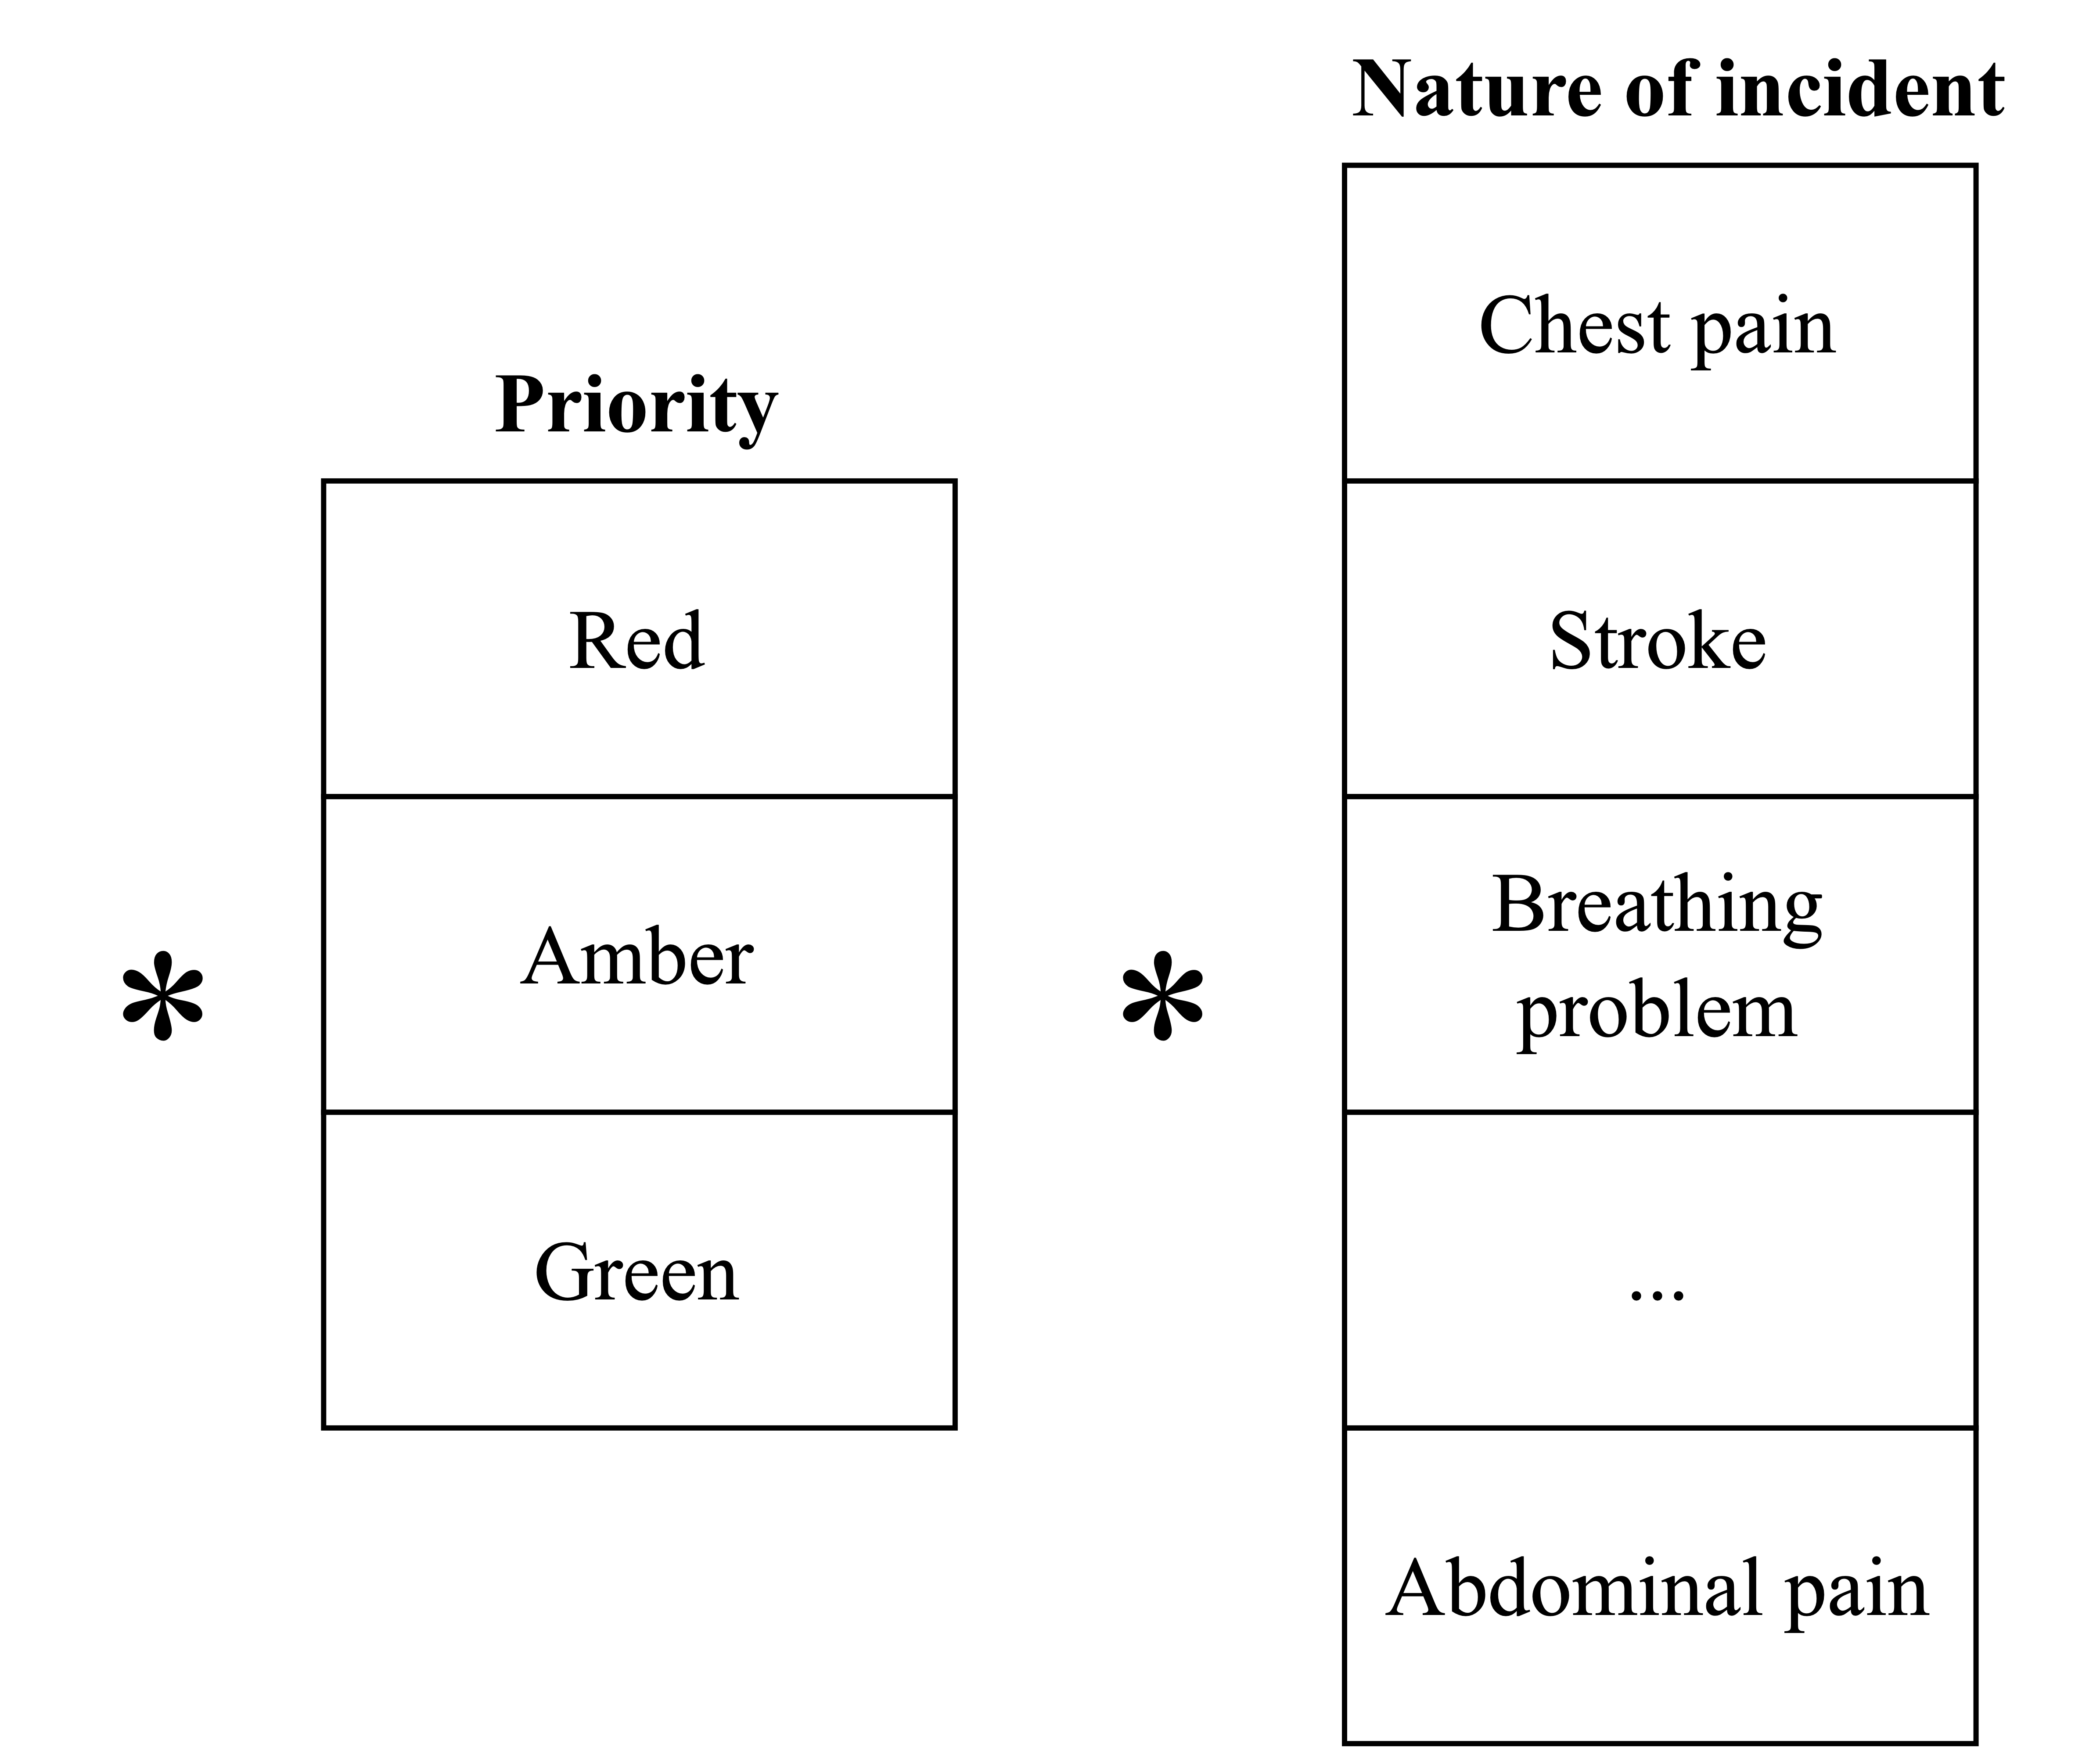
\includegraphics{/Users/bahmanrostami-tabar/Documents/1-research/1-research_papers/Work with Rob Hyndman/forecasting-emergency-medcine/img/group.png}

}

}

\subcaption{\label{fig-hierarchy-2}Grouped structure: Incidents could be
grouped into priority (i.e.~Red, Amber \& Green) and the nature of
attended incident (i.e.~there are 35 different nature of incidents
including chest pain , breathing problems, heart attack, stroke, and so
on). The symbol * refers to the crossed attributes between hierarchical
and grouped levels.}
\end{minipage}%

\caption{\label{fig-hierarchy}The hierarchical and grouped structure of
attended incidents (ambulance demand).}

\end{figure}

Table~\ref{tbl-hierarchy} also displays the structure of data with the
total number of series at each level. At the top level, we have the
total attended incidents for the country. We can split these total
attended incidents by control area, by health board, by priority or by
nature of incident. There are 3 control areas breakdown by 7 local
health boards. Attended incident data are categorized into 3 priority
classes of red, amber and green. There are also 35 different nature of
incidents such as chest pain, stroke, breathing problem, etc. In total,
across all levels of disaggregation, there are 1530 time series.

\hypertarget{tbl-hierarchy}{}
\begin{table}
\caption{\label{tbl-hierarchy}Number of time series in each level for the hierarchical \& grouped
structure of attended incidents }\tabularnewline

\centering
\begin{tabular}{lr}
\toprule
Level & Number of series\\
\midrule
All country & 1\\
Control & 3\\
Health board & 7\\
Priority & 3\\
Priority * Control & 9\\
\addlinespace
Priority * Health board & 21\\
Nature of incident & 35\\
Nature of incident * Control & 105\\
Nature of incident * Health board & 245\\
Priority * Nature of incident & 104\\
\addlinespace
Control * Priority * Nature of incident & 306\\
Control * Health board * Priority * Nature of incident (Bottom level) & 691\\
Total & 1530\\
\bottomrule
\end{tabular}
\end{table}

Given the total number of time series, direct visual analysis is
infeasible. Therefore, we first compute features of all 1530 time series
\citep{m3pca} and display the strength of trend and weekly seasonality
strength in Figure~\ref{fig-feature}. Each point represents one time
series with the strength of trend in x-axis and the strength of
seasonality in y-axis. It is clear that there are some series showing
strong trends and/or seasonality, corresponding to series at the higher
levels of the hierarchy. The majority of series show low trend and
seasonality. These are time series belonging to the bottom series,
series related to the nature of incidents for a given control, health
board and priority level. Bottom series are dominated by noise with
little or no systematic patterns.

\begin{figure}

{\centering \includegraphics[width=0.7\textwidth,height=\textheight]{main_files/figure-pdf/fig-feature-1.pdf}

}

\caption{\label{fig-feature}Time series features of attended incidents
across all levels (1530 series)}

\end{figure}

In addition to displaying the trend and seasonality features, we also
visualize few time series at various levels of the aggregation.
Figure~\ref{fig-dataviz2} reveals different information such as trend,
seasonality and noise. For example, some series depict seasonality and
trend, whereas some other series report low volume of attended incidents
and entropy, making them more volatile and difficult to forecast. At the
level on nature of incidents combined with categories of other levels,
there are many series that contain zeros with low counts. As such, the
data set represents a diverse set of daily time series patterns.

\begin{figure}

{\centering \includegraphics[width=1\textwidth,height=\textheight]{main_files/figure-pdf/fig-dataviz2-1.pdf}

}

\caption{\label{fig-dataviz2}Time series of attended incidents at
various levels.}

\end{figure}

We consider several forecasting models that account for the diverse
patterns of the time series across the entire hierarchy. In developing
the forecasting models, the time series of holidays are also used in
addition to the attended incidents. We use public holidays, school
holidays and Christmas Day and New Year's Day as predictors of incident
attended. These type of holidays will affect peoples' activities and may
increase or decrease the number of attended incidents.

\hypertarget{forecasting-methods}{%
\subsection{Forecasting methods}\label{forecasting-methods}}

Given the presence of various significant patterns in the past attended
incidents, we consider three different forecasting models to generate
the base forecasts. Once the base forecasts are produced, hierarchical
and grouped time series methods are used to reconcile them across the
all levels. We briefly discussed forecasting models in the following
sections, and the hierarchical forecasting methods are discussed in
Section~\ref{sec-htc}.

\textbf{Naive:} We start with a simple forecasting approach, assuming
that the future days will be similar to past days. We use the empirical
distribution of the past daily attended incidents to create the forecast
distribution of future attended incidents. We consider the empirical
distribution of the most recent year of historic data on a rolling basis
to capture potential changes in behavior over
time.\todo{Actually we use all the data.}

\textbf{Exponential Smoothing State Space model (ETS):} ETS models
\citep{hyndman2021forecasting} can combine trend, seasonality and error
components in a time series through various forms such as additive,
multiplicative or mixed. The trend component can be none (``N''),
Additive (``A''), damped (``Ad'') or multiplicative (``M''). The
seasonality can be none (``N''), Additive (``A''), or multiplicative
(``M''). The error term can also be additive (``A'') or multiplicative
(``M''). To forecast the attended incidents at each level, we use the
\texttt{ETS()} function in the \texttt{fable} package \citep{fable2022}
in R. To identify the best model for a given time series, the ETS
function uses the corrected Akaike's Information Criterion (AICc).

Despite the popularity and the relevance of automatic \texttt{ETS} in
this study, however it may produce forecast distributions that are
non-integer and include negative values, despite the number of attended
incidents being integer and non-negative. When using \texttt{ETS}, a
time series transformation approach could be used to generate strictly
positive forecasts, although forecast distributions will still be
non-integer. An alternative is to use forecasting models that produce
integer, non-negative forecasts. in the following section we present
Generalized Linear Models (GLMs) and Poisson Regression to produce count
base forecasts.

\textbf{Generalized Linear Model (GLM):} GLMs are a family of models
developed to extend the concept of linear regression models. They
perform a regression by modeling the response variable as coming from a
particular member of the exponential family, and then transforming the
mean of the response so that the transformed mean is a linear function
of the predictors. One of the models that is frequently used in practice
to generate count forecasts is the Poisson regression. We will consider
forecasting attended incidents using the covariates spline trend, day of
the week dummy variables (from Monday to Sunday), Fourier terms to
capture yearly seasonality, public holidays (1 when is public holiday, 0
otherwise), school holidays (1 when is school holiday, 0 otherwise) and
Christmas Day (1 when is Christmas Day, 0 otherwise) and New Year's Day
(1 when is New Year's Day, 0 otherwise). We fit a Poisson regression
model using the function \texttt{glm()} from the package in R, with the
argument \texttt{family\ =\ poisson} to specify that we wish to fit a
Poisson regression model.

\textbf{Poisson Regression using tscount: } We consider another Poisson
regression model that takes into account serial dependence in addition
to covariates used in the GLM model. To that end, we use
\texttt{tsglm()} function in \emph{tscount} package in R
\citep{JSSv082i05} to model the attended incidents. The logarithmic link
function is used to ensure that the parameter of Poisson distribution is
always positive. This model can be estimated via maximization of the
likelihood function based on Poisson mass function. The regression model
captures the short range serial dependence by including the three order
autoregressive terms.

\textbf{Ensemble method:} we also use an ensemble method that combines
forecasts generated from Naive, ETS, GLM and Poisson regression to form
a mixture distribution \citep{combinations}.

\hypertarget{performance-evaluation}{%
\subsection{Performance evaluation}\label{performance-evaluation}}

To evaluate the performance of the various forecasting approaches, we
split the data into a series of ten training and test sets. We use a
time series cross-validation approach \citep{hyndman2021forecasting},
with a forecast horizon of 84 days, and each training set expanding in
42-day steps. The first training set uses all data up to 2018-04-25, and
the first test set uses the 84 days beginning 2018-04-26. The second
training set uses all data up to 2018-06-06, with the second test set
using the following 84 days. The largest training set ends on
2019-05-09, with the test set ending on 2019-07-31. Model development
and hyper-parameter tuning is performed using the training data only.
Forecasting performance is evaluated using both point and probabilistic
error measures. While we compute forecast errors for the entire 12
weeks, we are most interested in the last 42 days of each test set,
because that corresponds to how forecasts are generated for planning in
practice. Forecasting performance is evaluated using both point and
probabilistic error measures.

Point forecast accuracy is measured via the Mean Squared Scaled Error
(MSSE) and the Mean Absolute Scaled Error (MASE). The Mean Absolute
Scaled Error (MASE) \citep{HK06} is calculated as: \[
  \text{MASE} = \text{mean}(|q_{j}|),
\] where \[
  q_{j} = \frac{ e_{j}}
    {\displaystyle\frac{1}{T-m}\sum_{t=m+1}^T |y_{t}-y_{t-m}|},
\] and \(e_{j}\) is the point forecast error for forecast horizon \(j\),
\(m = 7\) (as we have daily seasonal series), \(y_t\) is the observation
for period \(t\), and \(T\) is the sample size (the number of
observations used for training the forecasting model). The denominator
is the mean absolute error of the seasonal naive method in the fitting
sample of \(T\) observations and is used to scale the error. Smaller
MASE values suggest more accurate forecasts. Note that the measure is
scale-independent, thus allowing us to average the results across
series.

A related measure is MSSE \citep{hyndman2021forecasting}, which uses
squared errors rather than absolute errors:
\begin{equation}\protect\hypertarget{eq-RMSSE}{}{
  \text{MSSE} = \text{mean}(q_{j}^2),
}\label{eq-RMSSE}\end{equation} where, \[
  q^2_{j} = \frac{ e^2_{j}}
    {\displaystyle\frac{1}{T-m}\sum_{t=m+1}^T (y_{t}-y_{t-m})^2},
\] Again, this is scale-independent, and smaller MSSE values suggest
more accurate forecasts.

To measure the forecast distribution accuracy, we calculate the
Continuous Rank Probability Score \citep{gneiting2014probabilistic}. It
rewards sharpness and penalizes miscalibration, so it measures overall
performance of the forecast distribution.
\begin{equation}\protect\hypertarget{eq-CRPS}{}{
  \text{CRPS} = \text{mean}(p_j),
}\label{eq-CRPS}\end{equation} where \[
  p_j = \int_{-\infty}^{\infty} \left(G_j(x) - F_j(x)\right)^2dx,
\] where \(G_j(x)\) is the forecasted probability distribution function
for forecast horizon \(j\), and \(F_j(x)\) is the true probability
distribution function for the same period.

\hypertarget{sec-htc}{%
\section{Hierarchical and grouped time series forecasting
techniques}\label{sec-htc}}

There are many applications in the healthcare and in particular in EMS
where a collection of time series is available. These series are
generally hierarchically organized based on multiple levels such as
area/region, health board and/or are aggregated at different levels in
groups based on nature of demand, priority of demand or some other
attributes. While series could be strictly hierarchical or only grouped
bases on some attributes, in many situation a more complex structures
arise when attributes of interest are both nested and crossed, having
hierarchical and grouped structure. This is also the case as discussed
in Section~\ref{sec-data}.

\hypertarget{independent-base-forecast}{%
\subsection{Independent (base
forecast)}\label{independent-base-forecast}}

A common practice in healthcare (and EMS) to predict hierarchical and
grouped series relies on producing independent forecast, also refereed
to as base forecast, typically by different teams as the need for such
forecasts arise. This is also known as base forecast. We observe \(n\)
time series at time \(t\), across the entire hierarchical and grouped
structure, written as \(y_t\). The base forecasts of \(y_{T+h}\) given
data \(y_1,\dots,y_T\) are denoted by \(\hat{y}_h\) for h steps-ahead
for all \(n\) series (\(n=1530\) in this study). Forecasts generated in
this way are nor coherent.

\hypertarget{reconciliation-methos}{%
\subsection{Reconciliation methos}\label{reconciliation-methos}}

Traditionally, alternative approaches to produce coherent forecasts for
hierarchical and grouped time series involves using bottom-up and
top-down methods by generating forecasts at a single level and then
aggregate or disaggregate. Top-down requires having a unique structure
to disaggregated forecasts generated at top level by proportions.
However, given that we have multiple grouped attributes combined with
the hierarchical structure, there is no unique way to disaggregate top
forecast. Hence the top-down can not be used in this case, so either we
can do some kind of reconciliation or must define our own top-down
method for each hierarchy. The recommended approach is to use
reconciliation. In the following sections, we first discuss some
notations and then present bottom-up and forecast reconciliation
approach used in this study to generate coherent forecasts.

\hypertarget{notations}{%
\subsubsection{Notations}\label{notations}}

Let \(b_t\) be a vector of \(n_b\) ``bottom-level'' time series at time
\(t\), and let \(a_t\) be a corresponding vector of \(n_a = n-n_b\)
aggregated time series, where

\[
 a_t = Ab_t
\]

and \(A\) is the \(n_a\times n_b\) ``aggregation'' matrix specifying how
the bottom-level series \(b_t\) are to be aggregated to form \(a_t\).
The full vector of time series is given by \[
 y_t = \begin{bmatrix}a_t \\b_t\end{bmatrix}.
\] This leads to the \(n\times n_b\) ``summing'' or ``structural''
matrix given by \[
  S = \begin{bmatrix}A \\ I_{n_b}\end{bmatrix}
\] such that \(y_t = Sb_t\).

\hypertarget{bottom-up-bu-and-linear-reconciliation-methods}{%
\subsubsection{Bottom-up (BU) and linear reconciliation
methods}\label{bottom-up-bu-and-linear-reconciliation-methods}}

Bottom-Up is a simple approach to generate coherent forecasts. It first
involves creating the base forecasts for the bottom level series. These
forecasts are then aggregated to the upper levels which results in
generating coherent forecasts. BU approach can capture the dynamics of
the series at the bottom level, but they may be noisy and difficult to
forecast as well. BU approach is limited on using only forecasts at the
bottom level and does not utilize all the information available across
the hierarchical and grouped structure. Forecast reconciliation
approaches fill this gap and combine and reconcile all the base
forecasts in order to produce coherent forecasts.

Given the summing matrix and base forecasts, bottom-up and linear
reconciliation methods can be written as \(\tilde{y}_h = SG\hat{y}_h\)
for different matrices \(G\).

Optimal reconciled forecasts are obtained with
\(G=(S'W^{-1}S)^{-1}W^{-1}\), or \(\tilde{y}_h = M\hat{y}_h,\) where the
\(n\times n\) ``mapping'' matrix is given by
\(M = S(S'W^{-1}S)^{-1}W^{-1},\) where \(\hat{y}_h\) are the \(h\)-step
forecasts of \(y_{T+h}\) given data to time \(T\), and \(W\) is an
\(n \times n\) positive definite matrix. Different choices for \(W\)
lead to different solutions such as Ordinary Least Square (OLS) ,
Weighted Least Square (WLS) and Minimum Trace (MinT)
\citep{WicEtAl2019}. We use the implementation of these methods in the
fable package in R in the experiment.

\hypertarget{sec-result}{%
\section{Results and discussion}\label{sec-result}}

In this section, we compare the forecasting performance of Naive, ETS,
GLM, Tscount and the ensemble model using base forecast and Minimum
Trace (Mint) methods. We have also computed the forecast accuracy for
Ordinary Least Square (OLS) and Weighted Least Square (WLS) approaches.
However, they are not reported here because their accuracy is
outperformed by Mint. We should also note that forecasts, and
consequently their corresponding errors, are generated for the entire
hierarchy and they could be reported at any level, if required.

The overall forecasting performance is reported in
Table~\ref{tbl-result}, in which the average forecast accuracy per
model, method and the hierarchical level is presented. Reported forecast
accuracy are averaged across all forecast horizons, rolling origins and
series at each level. Table~\ref{tbl-result} presents both point and
probabilistic forecast accuracy at total, control area, health board and
bottom level series. Point forecast performance are reported using MASE
and RMSSE in Table~\ref{tbl-result-1} and Table~\ref{tbl-result-2},
respectively. Probabilistic forecast accuracy is reported using CRPS in
Table~\ref{tbl-result-3}. The bold entries in each table identify a
combination of method and model that performs best for the corresponding
level (i.e.~each column), based on the smallest values of accuracy
measures.

Table~\ref{tbl-result-1} shows that forecast reconciliation (i.e.~Mint)
improves forecast accuracy at the higher levels of the hierarchy
including total, control area and health board. However, it is does not
result in accuracy improvement at the bottom level series, fro which
base forecasts are more accurate. This might be due to the noisy
structure of time series at the bottom level and the fact that base
forecasts produced for the bottom of hierarchy are from well-specified
forecasting models and therefore does not gain benefit from forecast
reconciliation. Generally, if the bottom-level series are sufficiently
smooth, base forecast is expected to outperform hierarchical
reconciliation due to the better forecasts available at the level. It is
also clear from Table~\ref{tbl-result-1} that the ensemble method
improves forecast accuracy at total, control area and health board.
However, this does not remain valid for bottom series where the Poisson
regression by GLM outperforms other approaches.

Table~\ref{tbl-result-2} also reports point forecast accuracy but using
RMSSE. The outperformance of forecast reconciliation using Mint at
higher levels of hierarchy is also confirmed by RMSSE. However, for the
bottom series, we observe that the base forecasts generated by ETS are
the most accurate, followed by its reconciliations forecasts.

\begin{table}

\caption{\label{tbl-result}Average forecast perfomance calculated on
out-of-sample with time series cross validation applied to attended
incident data. The best approach is highlighted in
bold.}\begin{minipage}[t]{\linewidth}
\subcaption{\label{tbl-result-1}Point forecast accuracy using MASE }

{\centering 

\tabularnewline

\centering
\begin{tabular}[t]{llllll}
\toprule
\multicolumn{2}{c}{ } & \multicolumn{4}{c}{MASE} \\
\cmidrule(l{3pt}r{3pt}){3-6}
method & model & Total & Control areas & Health boards & Bottom\\
\midrule
base & ensemble & 0.7543 & 0.8432 & 0.8648 & 1.004\\
base & ets & 0.9360 & 0.9133 & 0.8884 & 1.031\\
base & iglm & 0.8609 & 0.9083 & 0.9039 & \textbf{0.999}\\
base & naiveecdf & 1.1396 & 1.0633 & 1.0389 & 1.017\\
base & tscount & 0.8704 & 0.9109 & 0.9041 & 1.000\\
\addlinespace
mint & ensemble & \textbf{0.7332} & \textbf{0.8346} & \textbf{0.8621} & 2.251\\
mint & ets & 0.8593 & 0.9001 & 0.8997 & 1.258\\
mint & iglm & 0.8176 & 0.8805 & 0.8883 & 2.490\\
mint & naiveecdf & 1.1395 & 1.0631 & 1.0389 & 2.648\\
mint & tscount & 0.8218 & 0.8846 & 0.8913 & 2.516\\
\bottomrule
\end{tabular}

}

\end{minipage}%
\newline
\begin{minipage}[t]{\linewidth}
\subcaption{\label{tbl-result-2}Point forecast accuracy using RMSSE }

{\centering 

\tabularnewline

\centering
\begin{tabular}[t]{llllll}
\toprule
\multicolumn{2}{c}{ } & \multicolumn{4}{c}{RMSSE} \\
\cmidrule(l{3pt}r{3pt}){3-6}
method & model & Total & Control areas & Health boards & Bottom\\
\midrule
base & ensemble & 0.7338 & 0.8335 & 0.8652 & 0.9885\\
base & ets & 0.9465 & 0.9126 & 0.8915 & \textbf{0.9795}\\
base & iglm & 0.8383 & 0.9073 & 0.9125 & 0.9958\\
base & naiveecdf & 1.0559 & 1.0213 & 1.0188 & 1.0081\\
base & tscount & 0.8446 & 0.9090 & 0.9114 & 1.0069\\
\addlinespace
mint & ensemble & \textbf{0.7153} & \textbf{0.8244} & \textbf{0.8621} & 1.2405\\
mint & ets & 0.8510 & 0.9002 & 0.9027 & 0.9879\\
mint & iglm & 0.8015 & 0.8814 & 0.8972 & 1.3379\\
mint & naiveecdf & 1.0558 & 1.0211 & 1.0188 & 1.4429\\
mint & tscount & 0.8020 & 0.8849 & 0.9003 & 1.3515\\
\bottomrule
\end{tabular}

}

\end{minipage}%
\newline
\begin{minipage}[t]{\linewidth}
\subcaption{\label{tbl-result-3}Probabilistic forecast accuracy using CRPS }

{\centering 

\tabularnewline

\centering
\begin{tabular}[t]{llllll}
\toprule
\multicolumn{2}{c}{ } & \multicolumn{4}{c}{CRPS} \\
\cmidrule(l{3pt}r{3pt}){3-6}
method & model & Total & Control areas & Health boards & Bottom\\
\midrule
base & ensemble & 12.44 & 5.681 & 3.385 & 0.2421\\
base & ets & 13.96 & 5.974 & 3.430 & 0.2422\\
base & iglm & 14.49 & 6.061 & 3.488 & 0.2420\\
base & naiveecdf & 30.35 & 10.887 & 5.445 & 0.3000\\
base & tscount & 14.98 & 6.124 & 3.500 & 0.2429\\
\addlinespace
mint & ensemble & \textbf{12.09} & \textbf{ 5.664} & \textbf{3.383} & 0.2455\\
mint & ets & 13.28 & 5.884 & 3.472 & \textbf{0.2412}\\
mint & iglm & 13.35 & 5.812 & 3.394 & 0.2443\\
mint & naiveecdf & 30.36 & 10.904 & 5.446 & 0.3103\\
mint & tscount & 13.55 & 5.868 & 3.423 & 0.2483\\
\bottomrule
\end{tabular}

}

\end{minipage}%

\end{table}

Table~\ref{tbl-result-2} presents the accuracy of the forecast
distributions measures by CRPS, which considers both forecasting
reliability and interval sharpness. The smaller the value of CRPS, the
better the comprehensive performance. We observe that forecast
reconciliation results in forecast improvement, regardless of the
hierarchical level. Ensemble method is also more accurate fore higher
levels, but ETS performs better at the bottom level. While results show
that forecast reconciliation does not improve point forecast at the
bottom level, however Table~\ref{tbl-result-2} indicates that it
generates more accurate forecasts than base method. The outperformance
of probabilistic forecast reconciliation at the bottom level may
highlight an important fact. The reconciliation method may improve
forecast accuracy at certain number of quantiles at the tails of
forecast distribution, which are critical for managing risks.

Overall, our results indicate that forecast reconciliation using MinT
method provides reliable forecasts, and all methods that reconcile using
information at all levels of the forecast improve upon base
(unreconciled) forecasts, except the bottom level series. For bottom
series with less obvious patterns, base forecasts near center of
forecast distribution might be more accurate, while forecast
reconciliation using Mint could improve accuracy in the tails of of the
distribution.

In addition to the overall forecast accuracy presented in
Table~\ref{tbl-result}, we also report the point and probabilistic
forecast accuracy measures for each forecast horizon in
Figure~\ref{fig-accuracy}. The figure focuses on the hierarchical levels
important for decision making including total, control area and health
board, however this could be calculated for any level. We only
illustrate the results of the Mint method, given the its outperformance
described in Table~\ref{tbl-result}. For the illustration purpose, we
report the average weekly forecast accuracy instead of the daily
forecast horizon (i.e.~84 days including freezed planning (7 weeks = 42
days) plus future planing period (7 weeks = 42 days). Therefore, x-axis
shows horizons from week 1 (h= 1,\ldots,7) to week 12 (h= 78,\ldots,84).
The forecast horizon from week 7 to week 12 corresponds to the upcoming
planning horizon, which is used by planners and decision making. For the
point forecast, we can see that ensemble model performs much better than
others regardless of forecast horizons. For the probabilistic forecasts,
the distinction between forecasting models is less obvious. It is
important to highlight that, all forecasting models outperform the Naive
empirical distribution that is used as a Benchmark for both point and
probabilsitic forecasts.

\begin{figure}[H]

{\centering \includegraphics[width=1\textwidth,height=\textheight]{main_files/figure-pdf/fig-accuracy-1.pdf}

}

\caption{\label{fig-accuracy}Average accuracy by week for 12 weeks. CRPS
is relative to a naive ECDF. MASE and MSSE are relative to the
corresponding values for the training set.}

\end{figure}

\hypertarget{sec-conclusion}{%
\section{Conclusion}\label{sec-conclusion}}

Forecasting problems at Emergency Medical Services have often inherent
hierarchical and grouped structures. For example, looking at time series
of arrival calls in a clinical desk service, verified incidents, or
attended incidents in a country, they could be disaggregated by various
attributes of interest. Total demand in the country could be
disaggregated by region, then within each region by health board, within
each health board, by station/hospital, and so on down to the post code
area. Alternative structure may arise when attributes of interest are
crossed rather than nested. For example, the total demand could be
disaggrgated by priority (e.g Red, Amber, Green) or nature of incidents.
It is also natural to have a mixed structures, for example the total
demand could be disaggregated by priority and also by health board.

Despite the inherent hierarchical structure of the forecasting problem
in EMS, the common practice is to produce point forecast for each time
series independently. This practice may lead to the lack of coordination
and possibly undesirable and conflicting outcomes. Furthermore, due to
the asymmetric impact of resource allocation in this area, quantifying
forecast uncertainty through probabilistic forecasts is also of value as
it enables planners to manage associated risks. In this paper, we
investigate the application of hierarchical forecasting methods for
producing a probabilistic forecast of daily incident attended up to 84
days ahead, using different forecasting methods.

Our results indicates that forecast reconciliation can not only
contribute to a more coordinated efforts through producing coherent
forecasts when it comes to using forecasting to inform decisions in EMS,
but also it can result in forecast accuracy improvement. Our proposed
forecasting models combined with reconciliation approaches outperform
the empirical distribution benchmark. We show that a substantial
forecast improvement can be achieved at higher levels of hierarchical
and grouped structure time series by applying forecast reconciliation
methods. When a point forecast is of interest at the bottom level of
series, we observe that reconciliation may not improve the forecast
accuracy, if the bottom series are noisy and lack systematic patterns.
However, forecast reconciliation may result in more forecast results for
bottom series, if we are interested in the tails of forecast
distribution rather than just center measures like mean (i.e.~point
forecast). Producing consistent forecast are also crucial for informing
planning activities, we also demonstrate that proposed models produce
consistent forecasts across all forecast horizons. Therefore, we
recommend that forecast recociliation approaches to be adopted for
routine use in EMS, whenever hierarchical and/or grouped time series
data need to be forecasted. Moreover, we found that using an ensemble
forecasting model, combining al models developed in this paper, instead
of using each individualy, works remarkably well for our mixed
hierarchical \& grouped stucture.

Further research could investigate the practical benefits of
probabilistic hierarchical forecasting in EMS. Linking forecasts with
its utilities (response time, resource utilisation, etc) can offer an
opportunity to maximise benefits through more holistic planning
approach. While, we generated count attend incident for the base
forecast usign Poisson regression models, however the reconciles
forecast is snot yet count. This could be also an avenue for further
research.


\renewcommand\refname{References}
  \bibliography{bibliography.bib}


\end{document}
